\chapter{\IfLanguageName{dutch}{Stand van zaken}{State of the art}}%
\label{ch:stand-van-zaken}
In de snel evoluerende wereld van technologie speelt de mainframe nog altijd een essentiële rol als krachtige en betrouwbare computerinfrastructuur. Het is de ruggengraat van talloze organisaties, variërend van grote bedrijven tot overheidsinstanties, die vertrouwen op mainframes voor het verwerken van bedrijfskritieke workloads. Met de opkomst van moderne applicatie-ontwikkeling en de behoefte aan automatisering van het software ontwikkelproces, hebben mainframes zich aangepast aan het veranderende landschap. Dit doen ze door het aanbieden van de DevOps werkwijze en geavanceerde technologieën zoals Git, Azure DevOps en IBM Dependency Based Build ook wel bekend als IBM DBB.
\\ \\
Deze literatuurstudie onderzoekt de samenstelling van mainframe-technologie, IBM Dependency Based Build, Azure DevOps en Git workflows als een krachtige combinatie om een brug te slaan tussen het legendarische mainframe-erfgoed en het moderne automatisatie-gedreven software ontwikkelproces. Het onderzoek verkent de essentie van mainframes en hun evolutie door de jaren heen, evenals de cruciale rol die ze blijven spelen in het ondersteunen van kritieke bedrijfsprocessen.
\\ \\
Daarnaast wordt er dieper ingegaan op IBM Dependency Based Build, een krachtige tool ontwikkeld door IBM om mainframes te verbinden met moderne DevOps tools zoals Azure DevOps en Git. De studie onderzoekt de kenmerken en voordelen van IBM DBB en hoe dat het mogelijk maakt om een mainframe landschap open te stellen tot de DevOps werkwijze om op die manier software te ontwikkelen op de wijze waarop veel moderne platformen dat ook doen.
\\ \\
Verder wordt de focus gelegd op Azure DevOps, een krachtige tool-set die onder andere Azure Repos en Azure Pipelines bevat. Beide zijn noodzakelijk voor een goede DevOps werkwijze op te zetten. De studie verkent de mogelijkheden van de tool-set, zoals de verschillende onderdelen ervan en hoe deze bijdragen aan een DevOps werkomgeving.
\\ \\
Tot slot komt ook Git workflows aan bod, dit is een manier van werken om zo de flow van het software ontwikkelproces te bepalen. Dit is noodzakelijk voor de integriteit van de software die ontwikkeld wordt te bewaren. Er wordt in de studie onderzocht wat een Git workflow is en welke het best aanleunt tegen de mainframe waarden die zo hoog aangeschreven staan zoals betrouwbaarheid, integriteit en veiligheid.
\\ \\
\section{De mainframe}
\label{sec:de mainframe}

\subsection{Etymologie van de term mainframe}
De term mainframe is afgeleid van het Engelse woord \enquote{frame}, dat in dit geval verwijst naar de behuizing of structuur van de computer. Het woord \enquote{main} duidt op de centrale rol van deze computer in een gegevensverwerkingsomgeving. Een mainframe was bedoeld als het belangrijkste systeem in een computerinstallatie, waar andere randapparatuur en terminals op waren aangesloten \autocite{IBM2024}.
\\ \\
De oorsprong van de term mainframe kan worden toegeschreven aan de evolutie van computersystemen van die tijd. In de beginjaren van mainframe werden ze meestal aangeduid als grote computers of elektronische rekenmachines. Naarmate de technologie vorderde en de computers krachtiger en complexer werden, ontstond de behoefte aan een specifieke term om deze geavanceerde systemen te beschrijven \autocite{IBM2024}.
\\ \\
\subsection{Historie van de IBM mainframe}
De IBM mainframe heeft een rijke geschiedenis die teruggaat tot de vroege dagen van de computertechnologie.
\\ \\
\subsubsection{IBM 701 Electronic Data Processing machine (1952)}
In 1952 werd de IBM 701 gelanceerd als een geavanceerde elektronische gegevensverwerkingsmachine. Het was ontworpen om wetenschappelijke berekeningen en gegevensverwerkingstaken uit te voeren en bood meer rekenkracht en geheugencapaciteit dan eerdere computersystemen aan \autocite{IBM2024a}.
\\ \\
De IBM 701 maakte gebruik van vacuümbuizen als belangrijkste elektronische componenten en kon ongeveer 10.000 optellingen per seconde uitvoeren. Het systeem werd voornamelijk gebruikt door overheidsinstanties, laboratoria en grote bedrijven voor complexe wetenschappelijke en technische berekeningen \autocite{IBM2024a}.
\\ \\
De IBM 701 markeerde een belangrijke ontwikkeling in de computertechnologie, aangezien het een van de eerste commercieel succesvolle computers was die specifiek werd ontworpen voor gegevensverwerking. Het opende de deur naar geavanceerdere computersystemen en legde de basis voor toekomstige mainframes \auocite{IBM2024a}.
\\ \\
\subsubsection{IBM System/360 (1964)}
De ontwikkeling van de IBM/360 begon in de late jaren 1950 als een ambitieus project binnen IBM om een nieuwe generatie computersystemen te creëren die compatibiliteit zouden bieden tussen verschillende modellen. Het doel was om een reeks computers te ontwikkelen die zowel kleinere als grotere organisaties kon bedienen \autocite{IBM2024b}.
\\ \\
Op 7 april 1964 werd de IBM/360 officieel geïntroduceerd en werd het de eerste commercieel succesvolle mainframe computerreeks. Het systeem bood een breed scala aan modellen met verschillende prestatieniveaus en configuraties, waardoor het aan de behoeften van verschillende organisaties kon voldoen \autocite{IBM2024b}.
\\ \\
De IBM/360 was revolutionair omdat het een gemeenschappelijke architectuur introduceerde die compatibiliteit bood tussen de verschillende modellen. Hierdoor konden klanten hun investeringen in software en hardware beschermen, omdat programma’s op meerdere systemen konden draaien. Het was ook een van de eerste computersystemen die gebruikmaakte van geïntegreerde schakelingen \autocite{IBM2024b}.
\\ \\
De IBM/360 had een enorme impact op de computerindustrie en droeg bij aan de standaardisatie van computerarchitectuur. Het systeem werd breed geadopteerd door bedrijven, overheden en academische instellingen over de hele wereld en legde de basis voor latere ontwikkelingen in de mainframe-technologie \autocite{IBM2024b}.
\\ \\
\subsubsection{IBM System/370 (1970)}
De IBM/370 werd gelanceerd als opvolger van de IBM/360 en introduceerde belangrijke technologische verbeteringen, waaronder een uitgebreidere instructieset, verbeterde virtualisatiemogelijkheden en grotere geheugencapaciteit. Deze verbeteringen maakten het systeem krachtiger en veelzijdiger \autocite{IBM2024c}.
\\ \\
Een belangrijk kenmerk van de IBM/370 was de ondersteuning voor virtual memory, waardoor meerdere programma’s tegelijkertijd konden uitgevoerd worden en gebruik maken van het beschikbare geheugen. Dit leidde tot verbeterde systeemprestaties en efficiënter gebruik van resources \autocite{IBM2024c}.
\\ \\
De IBM/370 mainframe werd breed gebruikt door bedrijven en overheidsinstanties voor diverse toepassingen, waaronder gegevensverwerking, transactionele systemen, wetenschappelijke berekeningen en databasebeheer. Het bood hogere prestaties en schaalbaarheid, waardoor het kon voldoen aan de groeiende behoeften van organisaties \autocite{IBM2024c}.
\\ \\
\subsubsection{IBM System ZSeries (2000)}
De IBM zSeries, gelanceerd in het jaar 2000, was een belangrijke mijlpaal voor de mainframe-industrie. Het bood verschillende baanbrekende kenmerken en voordelen die een grote impact hadden.
\\ \\
Een van de belangrijkste aspecten van de zSeries was de aanzienlijke verbetering in prestaties en schaalbaarheid. Het systeem was in staat om enorme werklasten te verwerken en te voldoen aan de groeiende behoeften van bedrijven. Dit maakte het een krachtige keuze voor organisaties die behoefte hadden aan grote rekenkracht en verwerkingscapaciteit \autocite{IBM2024d}.
\\ \\
Naast prestatieverbeteringen stond de zSeries bekend om zijn ongeëvenaarde betrouwbaarheid en beschikbaarheid. Het bevatte geavanceerde functies zoals redundantie, fouttolerantie en hot-swappable componenten. Deze kenmerken minimaliseerden ongeplande downtime en waarborgden een hoge beschikbaarheid van systemen, wat van cruciaal belang was voor bedrijfskritieke toepassingen \autocite{IBM2024d}.
\\ \\
Een ander belangrijk aspect van de zSeries was de ondersteuning voor moderne technologieën. Het introduceerde onder andere Linux op mainframes, waardoor organisaties zowel mainframe- als open source-technologieën op één platform konden gebruiken. Dit opende de deur voor een breed scala aan toepassingen en bood flexibiliteit in de ontwikkeling en implementatie van software \autocite{IBM2024d}.
\\ \\
Beveiliging is altijd een cruciale factor geweest in de mainframe-wereld, en de zSeries stelde op dit gebied niet teleur. Het bood geavanceerde beveiligingsfuncties, zoals ingebouwde encryptie, toegangscontrolemechanismen en auditmogelijkheden. Deze functies waarborgden de integriteit en vertrouwelijkheid van gegevens, wat essentieel is in omgevingen waar gevoelige informatie wordt verwerkt \autocite{IBM2024d}.
\\ \\
Een ander belangrijk voordeel van de zSeries was de mogelijkheid om naadloos te integreren met bestaande legacy-systemen en applicaties. Hierdoor konden organisaties waardevolle bedrijfsactiva behouden en moderniseren zonder de noodzaak van grootschalige herontwikkeling. Dit zorgde voor een soepele overgang naar de nieuwe technologie en minimaliseerde de verstoring van bestaande processen \autocite{IBM2024d}.
\\ \\
\subsubsection{Tijdlijn van de grootste IBM mainframes}
\color{gray}
\rule{\linewidth}{1pt}
    \ytl{1952}{IBM 701-de eerste commerciële mainframe van IBM}
    \ytl{1964}{IBM System/360-de eerste mainframe-reeks die compatibiliteit bood over meerdere modellen}
    \ytl{1970}{IBM System/370-deze mainframe bood nieuwe mogelijkheden zoals virtueel geheugen en verbeterde instructiesets}
    \ytl{1980}{IBM System/38-mainframe met microprocessoren en een nieuwe programmeertaal genaamd \enquote{CPF} (Control Program Facility)}
    \ytl{1985}{IBM ES/9000-ondersteuning voor geavanceerde besturingssystemen zoals MVS/ESA en VM/ESA}
    \ytl{1990}{IBM System/390-opvolger van System/370, met de focus op verbeterde prestaties, beveiliging en schaalbaarheid}
    \ytl{2000}{IBM zSeries-deze mainframe had betere ondersteuning voor internet en webgebaseerde toepassingen, en verbeterde virtualisatie- en partitioneringsmogelijkheden}
    \ytl{2005}{IBM System z9-de opvolger van de zSeries, met een focus op betere prestaties en beveiliging, en verbeterde virtualisatie- en partitioneringsmogelijkheden}
    \ytl{2010}{IBM zEnterprise System-een hybride mainframe dat zowel traditionele mainframe- als BladeCenter-technologie combineerde}
    \ytl{2015}{IBM z13-de opvolger van zEnterprise System, met verbeterde prestaties, beveiliging en betere ondersteuning voor cloud computing en big-data analyse}
    \ytl{2021}{IBM z15-deze mainframe kreeg betere ondersteuning voor hybride cloud-omgevingen en AI-workloads}
    \ytl{2023}{IBM z16-de nieuwste generatie mainframe van IBM, het biedt real-time AI-inferentie en is het eerste kwantumveilige systeem op de markt}
\rule{\linewidth}{1pt}
\\
\autocite{Elliot2015} \autocite{IBMa} \autocite{IBMb}
\\ \\
\subsection{Concurrentie op het mainframe platform}
\subsubsection{1960s}
In de jaren 1960 had IBM een dominante positie op de mainframe-markt. Ze waren de toonaangevende leverancier van mainframes en hun System/360-serie was een belangrijke mijlpaal in de computerindustrie. Echter, waren er ook andere belangrijke concurrenten die IBM uitdaagden. Burroughs Corporation was daar een van, met hun B5000-serie die bekend stond om zijn geavanceerde architectuur en programmeertaal. Control Data Corporation (CDC) was ook een belangrijke concurrent, met hun CDC 6600 die destijds bekend stond als ’s werelds snelste computer \autocite{Museum2024}.
\\ \\
\subsubsection{1970s}
In de jaren 1970 bleef IBM een dominante positie behouden op de mainframe-markt, maar er waren nieuwe concurrenten die uitdagingen boden. Een belangrijke concurrent was Digital Equipment Corporation (DEC), een bedrijf dat bekend stond om zijn minicomputers. DEC bracht echter ook mainframes op de markt, zoals de DECsystem-10 en DECsystem-20, die aantrekkelijk waren voor verschillende organisaties \autocite{Society2017}.
\\ \\
Een andere belangrijke speler was Honeywell, dat zijn eigen reeks mainframes aanbood, zoals de Honeywell 6000-serie. Deze systemen waren populair in sectoren zoals banken en overheidsinstanties \autocite{Society2017}.
\\ \\
Bovendien begonnen in de jaren 1970 ook nieuwe bedrijven, zoals Amdahl Corporation en Hitachi, de mainframe-markt te betreden. Amdahl Corporation, opgericht door een voormalige IBM-manager, bood mainframes aan die compatibel waren met IBM-systemen, maar tegen lagere prijzen \autocite{Society2017}.
\\ \\
\subsubsection{1980s}
Doorheen de jaren 1980 werd de concurrentie op de mainframe-markt intenser, met verschillende spelers die de dominante positie van IBM probeerden uit te dagen. Een van de grootste concurrenten was Digital Equipment Corporation (DEC), dat in deze periode zijn VAX-computers lanceerde. De VAX-systemen waren krachtige machines die in staat waren om complexe taken uit te voeren en werden populair in bedrijfsomgevingen \autocite{Society2017}.
\\ \\
Een andere opkomende concurrent was Amdahl Corporation, dat IBM-compatibele mainframes aanbood tegen lagere prijzen. Amdahl wist een aanzienlijk marktaandeel te veroveren en werd een belangrijke speler in de mainframe-industrie \autocite{Society2017}.
\\ \\
Ook Hewlett-Packard (HP) betrad de mainframe-markt met zijn HP 3000-serie. Deze systemen waren gericht op kleinere organisaties en boden een combinatie van mainframe-functionaliteit met de gebruiksvriendelijkheid van minicomputers \autocite{Society2017}.
\\ \\
Naast deze concurrenten zette IBM zelf ook belangrijke ontwikkelingen voort. In 1980 introduceerde IBM de IBM 3081-mainframeserie, die verbeterde prestaties bood ten opzichte van eerdere modellen. Later in het decennium lanceerde IBM de 3090-serie, die geavanceerde mogelijkheden bood, zoals verbeterde geheugencapaciteit en verwerkingssnelheid \autocite{Society2017}.
\\ \\
\subsubsection{1990s}
Gedurende de jaren ’90 was IBM nog altijd leider in de markt, maar er waren ook concurrenten die uitdagende alternatieven aanboden. Zoals Amdahl, dat bracht in deze periode de 9000-serie mainframes uit, die concurrerende prestaties en betrouwbaarheid boden \autocite{Ceruzzi2003}.
\\ \\
Een andere concurrent die ook al in de jaren '80 aanwezig was is Hitachi met zijn Hitachi Mainframe Systems. Deze systemen waren populair in de Aziatische markt en boden krachtige verwerkingsmogelijkheden en schaalbaarheid \autocite{Ceruzzi2003}.
\\ \\
Een opvallende ontwikkeling in de jaren 1990 was de opkomst van open systemen en de Unix-besturingssystemen. Sun Microsystems was een belangrijke speler met zijn Sun Enterprise-servers, die draaiden op het Solaris-besturingssysteem. Deze systemen werden vaak gebruikt voor zware reken- en databasetoepassingen \autocite{Ceruzzi2003}.
\\ \\
Daarnaast begon IBM zelf ook met het aanbieden van open-systemen op basis van de IBM RS/6000-architectuur, die het AIX-besturingssysteem draaiden. Deze systemen combineerden de kracht van mainframes met de flexibiliteit van open systemen \autocite{Ceruzzi2003}.
\\ \\
\subsubsection{2000s}
Bij het begin van het nieuwe millennium bleef IBM veruit de grootste speler in de mainframe-wereld. Toch waren er nog altijd geduchte concurrenten zoals Fujitsu, een Japans technologiebedrijf. Fujitsu bood zijn eigen lijn van mainframes aan, zoals de Fujitsu BS2000-serie, die bekend stond om zijn betrouwbaarheid en schaalbaarheid \autocite{LaMonica2004}.
\\ \\
Een andere uitdager was Hewlett-Packard (HP), dat de non-stop servers aanbood. Deze waren gericht op transactionele verwerking en waren populair in sectoren zoals banken en financiële dienstverlening \autocite{LaMonica2004}.
\\ \\
Naast deze gevestigde spelers begon de opkomst van cloud computing in de jaren 2000 de dynamiek in de mainframe-markt te veranderen. Bedrijven zoals AmazonWeb Services (AWS) en Google Cloud Platform (GCP) boden schaalbare en flexibele cloudinfrastructuur aan, waardoor organisaties een alternatief kregen voor het beheren van hun eigen mainframes \autocite{AWS} \autocite{Google}.
\\ \\
IBM speelde ook in op de opkomst van cloud computing en introduceerde zijn eigen mainframe-gebaseerde cloudoplossingen, zoals IBM Cloud en IBM Z als een Service. Deze diensten boden klanten de mogelijkheid om mainframe-functionaliteit te benutten in een cloudomgeving \autocite{IBM}.
\\ \\
\subsubsection{2010s}
In de jaren 2010 bleef IBM zijn dominante positie voort zetten in de mainframe-markt, met zijn IBM Z-systemen die bekend stonden om hun schaalbaarheid, beveiliging en betrouwbaarheid. IBM investeerde voortdurend in de ontwikkeling van nieuwe mainframe-technologieën en introduceerde regelmatig verbeterde versies van zijn mainframe-systemen \autocite{IBM2024d}.
\\ \\
Naast IBM waren er enkele andere spelers die zich in de mainframe-markt begaven. Een belangrijke concurrent was Oracle Corporation, dat zijn Engineered Systems-lijn aanbood, waaronder de Oracle SuperCluster en de Oracle Exadata Database Machine. Deze systemen combineerden high-performance hardware met geoptimaliseerde software en waren specifiek gericht op gegevensverwerking en databasebeheer \autocite{Oracle}.
\\ \\
Een andere opkomende trend in die periode was de verschuiving naar gevirtualiseerde en software gedefinieerde infrastructuren. Bedrijven zoals VMware, met zijn virtualisatieoplossingen, en OpenStack, met zijn open-source cloudbeheerplatform, begonnen aan populariteit te winnen. Hoewel deze technologieën niet rechtstreeks mainframe-gericht waren, boden ze alternatieve manieren om IT-infrastructuur te schalen en beheren. Bovendien speelden cloudproviders zoals Amazon WebServices (AWS), Microsoft Azure en Google Cloud Platform (GCP) een steeds grotere rol in de IT-industrie \autocite{Google} \autocite{AWS} \autocite{VMWare}.
\\ \\
\subsubsection{Heden}
In de hedendaagse markt is IBM nog altijd heer en meester met zijn IBM Z-systemen. Deze systemen zijn geoptimaliseerd voor high-performance computing, beveiliging, schaalbaarheid en worden nog steeds gebruikt door organisaties over de hele wereld voor kritieke workloads en bedrijfsprocessen.
\\ \\
Naast IBM hebben andere technologiebedrijven, zoals Fujitsu en Unisys, nog steeds een aanwezigheid in de mainframe-markt. Fujitsu biedt zijn BS2000-mainframes aan, die zich richten op betrouwbaarheid en schaalbaarheid. Unisys heeft zijn Clear-Path Libra- en Dorado-systemen die geschikt zijn voor bedrijfskritieke applicaties \autocite{Fujitsu} \autocite{Unisys}.
\\ \\
Een opvallende trend is de verschuiving naar hybride cloudarchitecturen en de opkomst van cloud-native technologieën. Bedrijven zijn op zoek naar manieren om mainframe-technologie te integreren met cloudoplossingen, zoals IBM Cloud, Amazon Web Services (AWS), Microsoft Azure en Google Cloud Platform (GCP). Dit stelt organisaties in staat om de schaalbaarheid, flexibiliteit en kostenefficiëntie van de cloud te benutten, terwijl ze nog steeds kunnen profiteren van de kracht en betrouwbaarheid van mainframes voor hun kritieke workloads \autocite{Google} \autocite{AWS}.
\\ \\
Een andere belangrijke ontwikkeling in de mainframe-markt is de focus op beveiliging. Met de groeiende dreiging van cyberaanvallen en gegevensinbreuken is dit een topprioriteit geworden voor organisaties. IBM Z-systemen hebben ingebouwde beveiligingsfuncties zoals IBM Secure Service Container en Secure Execution voor het beschermen van gevoelige gegevens en het voorkomen van ongeautoriseerde toegang \autocite{IBMa}.
\\ \\
\section{IBM Dependency Based Build}
\label{sec:IBM dependency based build}
In dit hoofdstuk wordt er beschreven wat IBM Dependency Based Build is en waarvoor het in dit onderzoek zal gebruikt worden. Er wordt ook besproken hoe IBM DBB werkt zowel op de voorgrond als op de achtergrond.
\\ \\
\subsection{Introductie tot IBM Dependency Based Build?}
\subsubsection{Geschiedenis}
Een van de eerste versies van DBB is versie 1.0.1, deze versie was uitgekomen in juni 2018 en had als nieuwe features over de initiële 1.0.0 versie dat het JCL kon submitten en een dat het object beheer door middel van eigenaarsrollen verbeterd is. Bij versie 1.0.1 werden ook nog eens 2 extra sample programma's geïntroduceerd namelijk PL/I Helloworld en DB2 Bind Sample in Mortgage Application.
\\ \\
Terwijl de versie van DBB in 2018 nog maar heel pril is worden er aan sneltempo versies met bijhorende extra features en verbeteringen uitgebracht. Zo is er op het einde van 2018 al een versie 1.0.3 uitgebracht die extra features zoals:
\begin{itemize}
    \item Versie 1.0.2
    \begin{itemize}
        \item Multi-thread build support
        \item Binary en load module kopie support
        \item ISPF interactieve gateway support voor TSOExec en ISPFExec
        \item Opvangen en opslaan van indirecte dependencies
        \item Automatische Groovy script caching
        \item Build properties kunnen opgebouwd zijn uit andere build properties
        \item DBB configuratie properties
        \item SMF record generatie
        \item DBB Build manager introductie
    \end{itemize}
    \item Versie 1.0.3
    \begin{itemize}
        \item SMF record generatie
        \item DBB Build manager introductie
    \end{itemize}

\end{itemize}
\\ \\
In 2019 blijven er op hetzelfde tempo nieuwe versies uitkomen, elk kwartaal wordt er een nieuwe versie uitgerold van DBB zo zit IBM tegen eind 2019 al aan versie 1.0.7.
De belangrijkste features zijn onder andere:
\begin{itemize}
    \item Versie 1.0.4
    \begin{itemize}
        \item zFS directories in DD statements
        \item FIPS 140-2 compliance
        \item Error en warning messages zijn nu te vinden in het knowledge center
        \item
    \end{itemize}
    \item Versie 1.0.5
    \begin{itemize}
        \item Tar/gzip file support voor dependencies
        \item Non-roundtrippable character detectie door de migratie tool
        \item Linux on IBM Z support
    \end{itemize}
    \item Versie 1.0.6
    \begin{itemize}
        \item Introducering van Z Open Automation Utilities (ZOAU)
        \item Support voor aanpassingen aan database schema
        \item Support voor Db2 voor z/OS
        \item YAML bestanden voor build configuraties
        \item Swagger API documentatie
    \end{itemize}
    \item Versie 1.0.7
    \begin{itemize}
        \item Toevoeging van nieuwe ZOAU functionaliteit
        \item File tagging support voor CopyToHFS commando
    \end{itemize}
\end{itemize}
\\ \\
Doorheen 2020 zwakte het aantal versie-updates af naar slechts 2, zo werd er een update in maart en in juni uitgebracht voor DBB. Respectievelijk versies 1.0.8 en 1.0.9 hiervan zijn er een aantal nieuwe features opgelijst:
\begin{itemize}
    \item Versie 1.0.8
    \begin{itemize}
        \item File tagging support voor het CopyToHFS commando bij non-ASCII en UTF-8 gecodeerde bestanden
        \item Nieuwe copy mode toegevoegd bij het CopyToHFS commando dat ASA carriage control characters behoudt
        \item Support om het CopyToPDS commando als een build stap te registreren in de build report
    \end{itemize}
    \item Versie 1.0.9
    \begin{itemize}
        \item Personal daemon beschikbaar als toevoeging op de bestaande shared daemon
    \end{itemize}
\end{itemize}
\\ \\
Het bleef wat betreft versie-updates heel stil in het jaar 2021 en 2022 al was er in 2022 nog een laatste versie-update voor versie 1.0x van DBB. Die update werd doorgevoerd in maart 2022 en bepaald tot op heden de huidige versie van DBB 1.0x:
\begin{itemize}
    \item Versie 1.0.10
    \begin{itemize}
        \item Apache Groovy 4.0 upgrade
    \end{itemize}
\end{itemize}
\autocite{IBM2022}
\\ \\
In oktober 2021 komt er een nieuwe versie uit van DBB namelijk de versie 1.1x, deze versie heeft 4 updates gekregen sinds zijn ontstaan, de updates zijn niet zo talrijk als in versie 1.0x. Met de laatste update van versie 1.1x in maart 2023 zit men aan de huidige versie van DBB 1.1x, er zijn nog updates uitgekomen in juni 2021, oktober 2021 en maart 2022. De belangrijkste features per versie zijn de volgende:
\begin{itemize}
    \item Versie 1.1.0
    \begin{itemize}
        \item DBB Web Applicatie beschikbaar als een Red Hat OpenShift Container Platform (OCP) cluster
        \item Integratie met z/OS Automated Unit Testing Framework (zUnit)
        \item Introducering van simpelere dependency resolution en impact analyse API's
    \end{itemize}
    \item Versie 1.1.1
    \begin{itemize}
        \item DBB Web Applicatie kan geïnstalleerd worden op een Red Hat OpenShift Cotainer Platform (OCP cluster) door middel van een operator
        \item Support voor \enquote{report only} mode tijdens het uitvoeren van DBB z/OS commando API's
        \item DBB source code scanner kan programma's met IBM MQ call statements herkennen
    \end{itemize}
    \item Versie 1.1.2
    \begin{itemize}
        \item DBB Web Applicatie User Interface
        \item Introducering van de SearchPathDependencyResolver en SearchPathImpactFinder klassen
    \end{itemize}
    \item Versie 1.1.3
    \begin{itemize}
        \item Apache Groovy 4.0 upgrade
    \end{itemize}
    \item Versie 1.1.4
    \begin{itemize}
        \item JSON Web Token (JWT) eenmalige inlog authenticatie
        \item Statisch build report in HTML bestand
        \item APAR verbeteringen
    \end{itemize}
\end{itemize}
\autocite{IBM2023}
\\ \\
De versie die gebruikt zal worden voor dit onderzoek is de versie 2.0.0, die maakt deel uit van DBB 2.0x en werd geïntroduceerd in oktober 2022 en kreeg zijn eerste en voorlopig recentste update in mei 2023 (2.0.1). Zoals vermeld zal dit onderzoek gebruik maken van DBB 2.0.0, de belangrijkste feature updates voor DBB 2.0x zijn als volgt:
\begin{itemize}
    \item Versie 2.0.0 (versie onderzoek)
    \begin{itemize}
        \item DBB toolkit geïnstalleerd op z/OS UNIX verbind direct met db2 databases
        \item DBB toolkit heeft support voor zowel Java 8 als Java 11
        \item DBB 2.0 toolkit heeft de Apache Log4J logging technologie vervangen door SLF4J
    \end{itemize}
    \item Versie 2.0.1
    \begin{itemize}
        \item Toevoeging van het JobExec commando
        \item Toevoeging RACF Group Configuratie
    \end{itemize}
\end{itemize}
\autocite{IBM2023a}
\\ \\
\subsubsection{Definitie}
IBM Dependency Based Build biedt de mogelijkheid aan om traditionele z/OS applicaties die ontwikkeld zijn in programmeer talen zoals Cobol, PL/I en Assembler te builden als onderdeel van een moderne DevOps pipeline. Het biedt een moderne, op scripttaal gebaseerde, automatisatie mogelijkheid dat kan gebruikt worden op z/OS. DBB is gebouwd als een stand-alone product waarvoor geen specifieke source code manager of pipeline automation tool nodig is \autocite{IBM2023b}.
\\ \\
\subsection{Technische aspecten van DBB}
\subsubsection{Hoe het werkt}
DBB bevat een Java Application Programming Interface, kortweg API, die het mogelijk maakt om taken op z/OS te ondersteunen en afhankelijkheidsinformatie te creëren en te gebruiken voor de broncode die wordt verwerkt. DBB bestaat uit een z/OS-gebaseerde toolkit die de API's, een afhankelijkheidsscanner en Apache Groovy bevat. Er zijn ook afzonderlijk verkrijgbare componenten, waaronder een webapplicatie die de afhankelijkheidsinformatie en bouwrapporten opslaat en beheert, en een set Apache Groovy-templates om het gebruik van de API's voor het bouwen van applicaties te demonstreren \autocite{IBM2021}.
\\ \\
\subsubsection{Architectuur van DBB}
De architectuur van DBB bestaat volgens \textcite{IBM2021a} uit acht onderdelen die elk hun eigen taak hebben en absoluut nodig zijn om de DBB build uit te voeren. Elk van deze onderdelen kan vervangen worden door een alternatief product, DBB is niet afhankelijk van eender welk merk of product.
\paragraph{Component 1: MVS bestandssysteem}
Het MVS bestandssysteem is nodig omdat het resultaat van de compile/link stap nog altijd PDS gebaseerd is en daardoor is zo'n bestandssysteem onmisbaar.
\paragraph{Component 2: DBB}
Vanzelfsprekend is het DBB product nodig om een DBB build uit te voeren, het product komt met een DBB toolkit, bijhorende Groovy build scripts en z/OS build API's die bijvoorbeeld de compile/link in goede banen leidt.
\paragraph{Component 3: DBB WebApp}
In de DBB WebApp worden vooral de metadata van afhankelijkheden en de build resultaten bijgehouden in een web server. Deze web server is verbonden met een database, dit kan op eender welke database maar er wordt aangeraden om in productie gebruik te maken van Db2.
\paragraph{Component 4: Rocket Git}
Rocket Git is nodig om de communicatie met een Git server te verzorgen en heeft ook de functionaliteit om aan code conversie te doen van ASCII naar EBCDIC.
\paragraph{Component 5: Enterprise Git server}
In deze enterprise Git server zal de main repository komen en daarin zitten alle bestanden die nodig zijn om een DBB build uit te kunnen voeren. Dit gaat dan vooral over properties bestanden en source code voor applicatie ontwikkeling taken en om de development pipeline te kunnen uitvoeren. In dit onderzoek zal er gebruikgemaakt worden van Azure Repos als enterprise Git server maar een alternatief is bijvoorbeeld om een eigen Git server op te zetten op een eigen Linux omgeving.
\paragraph{Component 6: Pipeline orchestrator}
Een DBB build pipeline heeft ook een pipeline orchestrator nodig, dit is gedistribueerde server gebaseerde software die ervoor zorgt dat de pipeline stappen uitgevoerd kunnen worden. Dit kan gaan over automatische testing, cloning van de repository, DBB build en andere geautomatiseerde taken. Deze orchestrator houdt ook informatie over de builds bij zoals build status en logs. Er wordt in dit onderzoek gebruik gemaakt van Azure Pipelines als pipeline orchestrator maar een alternatief is bijvoorbeeld Jenkins.
\paragraph{Component 7: Pipeline agent}
Deze agent is nodig om de pipeline orchestrator te laten runnen en communiceren met z/OS.
\paragraph{Component 8: App dev IDE}
Dit is de plaats waarin de applicatie ontwikkelaar zijn aanpassingen aan source code zal aanbrengen. Dit kan elke Git gebaseerde IDE zijn zoals IBM Developer for zOS (IDz) of Visual Studio Code. In dit onderzoek wordt er gebruik gemaakt van beide IDE's.
\\ \\
De architectuur heeft ook een workflow die het doorloopt, \textcite{IBM2021a} geeft aan dat in een standaard geval dit neerkomt op negen stappen van begin tot einde. De stappen worden in chronologische volgorde hieronder opgesomd.
\\ \\
De applicatie ontwikkelaar maat wijzigingen aan de source code van een applicatie en maakt gebruik van DBB user build om te verifiëren dat de wijzigingen goed compileren en om eventueel een aantal testen uit te voeren.
\\ \\
De applicatie ontwikkelaar gaat nadien de wijzigingen commiten/pushen naar de enterprise Git server. De Git server ontvangt de wijzigingen nadat een push of merge is gebeurd en gaat dan, automatisch of manueel, het signaal geven aan de pipeline orchestrator dat er een pipeline mag gestart worden.
\\ \\
Deze start op zijn beurt dan een job die wordt doorgegeven aan de agent in z/OS, de communicatie tussen de pipeline orchestrator en de pipeline agent kan gebeuren via SSH of Personal Acces Token (PAT). Dit onderzoek zal gebruik maken van Personal Acces Tokens om de communicatie tussen pipeline agent en pipeline orchestrator te verzorgen.
\\ \\
De eerste stap die de agent zal doen nadat die het start job signaal krijgt is om de source code/repository van de Git server te clonen op z/OS naar een working tree repository. Deze working tree repository zal dan gebruikt worden in de volgende stap door de Groovy build scripts die in werking treden doordat de agent de DBB build start.
\\ \\
Deze build scripts voeren een compile/link uit via de z/OS build API's en zorgen ervoor dat de verkregen of aangepaste load modules op de juiste plek terechtkomen in het MVS bestandssysteem.
\\ \\
Eenmaal dat de build compleet is worden de gegevens zoals de metadata van afhankelijkheden en het resultaat van de build verstuurd naar de DBB Web App die deze gegevens dan opslaat in zijn databank.
\\ \\
Tot slot krijgt ook de agent de logs en resultaten binnen en die stuurt die op zijn beurt dan weer door naar de pipeline orchestrator om ook daar bepaalde logs en gegevens bij te houden over het resultaat. Dit alles is ook visueel terug te vinden in figuur \ref{fig:dbb architectuur}.
\begin{figure}[h]
    \centering
    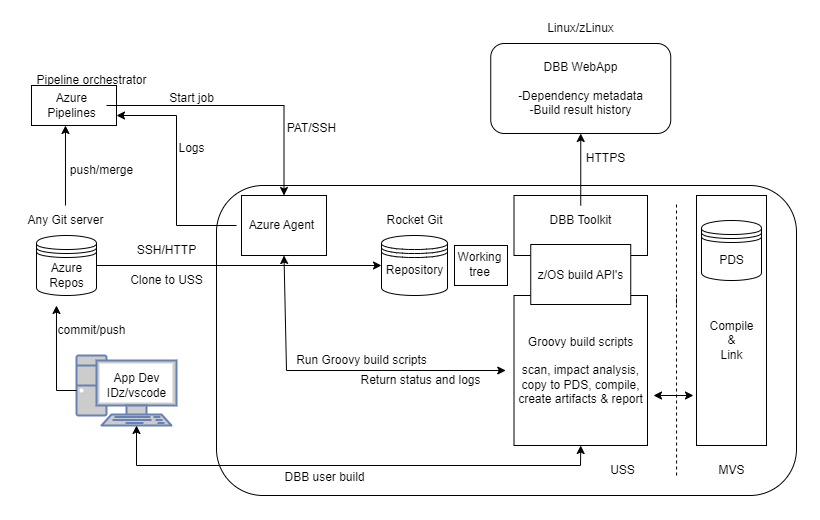
\includegraphics[scale=0.5]{DBB_architecture}
    \caption{DBB architectuur van dit onderzoek}
    \label{fig:dbb architectuur}
\end{figure}
\\ \\
\section{Azure DevOps}
\label{sec:azure devops}
\subsection{Wat is Azure DevOps?}
Volgens \textcite{Microsoft2024} ondersteunt Azure DevOps de samenwerking van ontwikkelaars, projectmanagers en medewerkers door een reeks processen aan te bieden die gebruikt worden om software te ontwikkelen. Het stelt organisaties in staat om sneller producten te maken en te verbeteren dan mogelijk is met traditionele softwareontwikkelingsmethoden.
\\ \\
Azure DevOps biedt geïntegreerde functies waartoe je toegang hebt via je webbrowser of IDE-client. Je kunt alle services gebruiken die bij Azure DevOps worden geleverd of alleen die services kiezen die je nodig hebt om je bestaande workflows aan te vullen.
\\ \\
\subsubsection{Azure producten}
Azure DevOps is een verzameling van vijf individuele services die samen de DevOps ontwikkel filosofie omarmt. Omdat de services onder de Azure DevOps suite zitten is communicatie tussen de services heel snel en heel eenvoudig op te zetten zonder gecompliceerde methodes om de communicatie tot stand te brengen.
\\ \\
Onder de \textcite{Microsoft2024} Azure DevOps suite zitten de volgende services:
\begin{itemize}
    \item Azure Boards: levert een suite van Agile tools om werk, code defecten en problemen te plannen en op te volgen, gebruikmakend van Kanban en Scrum methodes.
    \item Azure Repos: voorziet Git repositories of Team Foundation Version Control (TFVC) voor de source control van code.
    \item Azure Pipelines: voorziet build en release services om Continuous Integration (CI) en Continuous Delivery (CD) van applicaties te ondersteunen.
    \item Azure Test Plans: set van tools om applicaties te testen, inclusief manueel/exploratieve testing en continuous testing.
    \item Azure Artifacts: teams kunnen hier gebruik van maken om het delen van packages zoals Maven, npm, NuGet en andere packages van private- of publieke sources te integreren in pipelines.
\end{itemize}
Voor dit onderzoek zal er enkel gebruik gemaakt worden van de Azure Repos en Azure Pipelines services.
\\ \\
\subsection{Azure Repos als Source Code Control}
In Azure Repos zijn er twee manieren om aan Source Code Control te doen, via Team Foundation Version Control (TFVC) of via Git (gedistribueerd). TFVC is een gecentraliseerd client-server systeem. In zowel Git als TFVC kan er gebruik gemaakt worden van folders, branches en repositories om bestanden te organiseren. Voor dit onderzoek zal er gebruik gemaakt worden van een gedistribueerd Source Code Control (Git) \autocite{Microsoft2022}.
\\ \\
Via Azure Repos kan je alle repositories waartoe je toegang hebt beheren en eventueel aanpassen. Zo kunnen er branches, tags (versies), commits, pushes, merges en pull requests aangemaakt worden. Er kunnen ook handmatig, via Azure Repos, bestanden of folders geüpload worden \autocite{Microsoft2022}.
\\ \\
Azure Repos heeft ook de functionaliteit om automatisch of handmatig applicaties een nieuwe versie te bezorgen na een push. Zo kan er ook aan versiebeheer gedaan worden binnen Azure Repos, er kan ten allen tijden teruggegaan worden naar een vorige versie of commit. Op die manier hoef je niet expliciet meerdere versies bij te houden van eenzelfde applicatie en kan er bij problemen altijd teruggegaan worden naar een vorige werkende versie \autocite{Microsoft2022}.
\\ \\
Een ontwikkelaar die werkt met Azure Repos heeft een eigen kopie van de source repository op zijn computer. De source repository komt inclusief met alle branches en vorige versies van de repository. De ontwikkelaar werkt rechtstreeks op zijn eigen lokale repository en de aanpassingen worden gedeeld naar de centrale repository door een push naar de main source repository. Op die manier kan de ontwikkelaar zelf aan versiebeheer doen door de vorige versies te vergelijken met elkaar zonder netwerk connectie \autocite{Microsoft2022}.
\\ \\
Wanneer de ontwikkelaar een nieuw onderdeel wil toevoegen aan de applicatie kan die ook zijn eigen lokale branch maken om daarop verder te werken zonder andere ontwikkelaars te dwarsbomen. Doordat de branches lichtgewichten zijn op vlak van opslag kan er snel en makkelijk gewisseld worden tussen branches. Indien de ontwikkelaar klaar is met zijn onderdeel kan die door middel van een push/merge de main branch updaten met zijn nieuwe code, zo kan zijn lokale branch opgeruimd worden na de push/merge \autocite{Microsoft2022}.
\\ \\
\subsection{Azure Pipelines als pipeline orchestrator}
Azure Pipelines zorgt ervoor dat het mogelijk is om meerdere taken opeenvolgend te automatiseren om op die manier het builden en deployen van applicaties makkelijker en gestroomlijnder te maken. Met Azure Pipelines kan je taken zoals bestanden aanmaken en scripts of commando's uitvoeren, automatiseren in één of meerdere pipelines. Zo kan er met Azure Pipelines een systeem opgezet worden dat na afloop van een pipeline er opnieuw een pipeline zal gestart worden. Dit kan automatisch of manueel ingesteld worden. Het is ook mogelijk om Azure Pipelines je Git repository in Azure Repos te laten observeren en wanneer die een verandering detecteert in de source code, wordt er automatisch een pipeline gestart. Dit maakt het mogelijk om aan Continuous Integration (CI) te doen en doordat de mogelijkheid bestaat om meerdere pipelines/taken na elkaar uit te voeren kan er ook gedaan worden aan Continuous Delivery (CD). \autocite{Microsoft2023}
\\ \\
Een ontwikkelaar die werkt met Azure Pipelines hoeft, indien de optie CI aanstaat voor de repository en pipeline, enkel maar een push uit te voeren naar de repository en dan activeert die push de pipeline die daaraan gekoppeld is. De taken van de pipeline worden dan zelfstandig uitgevoerd zonder dat de ontwikkelaar zelf iets moet selecteren of uitvoeren. Er kan ook manueel een pipeline gestart worden, eenmaal gestart werkt die op dezelfde manier als de pipeline die geactiveerd werd door een push naar de gelinkte repository. \autocite{Microsoft2023}
\\ \\
Standaard is er ondersteuning om controle mechanismen in te schakelen binnenin de pipeline. Zo kan er voordat de pipeline effectief verandering brengt in bijvoorbeeld een productie applicatie eerst een review gevraagd worden aan een of meer leidinggevenden. Pipelines kunnen ook afgeschermd worden van bepaalde personen of groepen om zo confidentialiteit te waarborgen. \autocite{Microsoft2023}
\\ \\
Azure Pipelines hebben ook de mogelijkheid om automatische testing in gang te zetten bij het uitvoeren van de pipeline. Zo kan er naargelang het resultaat van de testen alsnog de wijziging van een applicatie afgebroken worden. Indien de pipeline succesvol beëindigd wordt kan er ook een optie aangevinkt worden om automatische versie controle aan te zetten. Zo kan er bij een applicatie van versie 1.0.1 na een succesvolle uitvoering van de pipeline de versie 1.0.2 meegegeven worden. \autocite{Microsoft2023}
\\ \\ \\ \\ \\ \\
\section{Git workflows}
\subsection{Software Development Lifecycle}
Een van de belangrijkste aspecten van mainframe software ontwikkeling is dat het betrouwbaar, beschikbaar en bruikbaar is. Deze workflow zit nagenoeg standaard ingebakken in mainframe softwareontwikkeling, maar hoe kan die workflow gerecreëerd of zelfs verbeterd worden door middel van gebruik te maken van Git om de softwareontwikkeling workflow op te stellen. Volgens Nelson \textcite{Lopez2023} is een van de beste strategieën om dezelfde eigenschappen van een mainframe workflow te bekomen om de Software Development Lifecycle te recreëren met behulp van Git, een Git ondersteunende IDE, CI pipeline, deployment policies en een CD pipeline.
\\ \\
Op de manier zoals voorgesteld door \textcite{Lopez2023} zou de source code storage niet meer in PDS's opgeslagen worden maar in een Git gedistribueerd bestandssysteem, versiebeheer zal niet meer verlopen via een SCM package ID maar via Git commit ID of Git tags. Indien er wijzigingen moeten aangebracht worden in de source code wordt er geen ISPF maar een IDE zoals VS-code of IDz, de compile/link van een programma zal dan weer verzorgd worden door een CI pipeline en niet door een JCL. Toestemmingen en het aanvaarden van wijzigingen aan applicaties zal je dan weer kunnen doen door middel van Git merge en deployment policies in plaats van de SCM. Als laatste zal het uiteindelijk deployen van een programma niet via JCL gebeuren maar via een CD pipeline.
\begin{figure}[h]
    \centering
    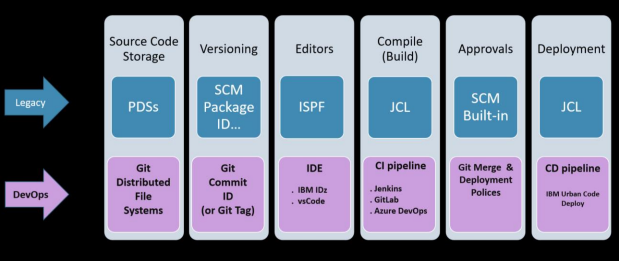
\includegraphics[scale=0.75]{Software_development_lifecycle}
    \caption{Software Development Lifecycle: Legacy vs DevOps \autocite{Lopez2023}}
    \label{fig:software development lifecycle}
\end{figure}
\\ \\ \\ \\
\subsection{Git branching strategie}
Elk bedrijf regelt zijn software ontwikkeling op een manier zodat er een duidelijk onderscheid en doel is voor elke omgeving. Zo is er een productieomgeving, de lopende versie van een applicatie zit daar te draaien. Er is ook een development omgeving waarin nieuwe features of verbeteringen voor die applicatie worden ontwikkeld. Tot slot is er ook nog de QA omgeving (Quality Assesment) deze omgeving wordt gebruikt om applicaties te testen op functioneel vlak vaak tegenover de productie database.
\\ \\
Om een goede branching strategie te bekomen is het belangrijk volgens \textcite{Lopez2023} dat tenminste die drie omgevingen worden geïmplementeerd als een branch in de branching strategie. Dit komt neer op een main (productie) branch, een develop (development/ontwikkeling) branch en een release (QA) branch.
\\ \\
Om nog beter te werk te gaan moeten er nog een aantal zaken toegevoegd worden aan de branching strategie zo heeft Nelson Lopez het onder andere over een feature en hotfix/nood branch. Die laatste is voor noodgevallen waarin er heel snel iets veranderd moet worden aan de applicatie die in productie draait. De feature branch zou dan weer een lokale branch worden waarin de ontwikkelaar werkt aan zijn opdracht voor die applicatie. De workflow die wordt beschreven door Nelson Lopez is visueel te vinden in figuur \ref{fig:git branching strategie}.
\begin{figure}[h]
    \centering
    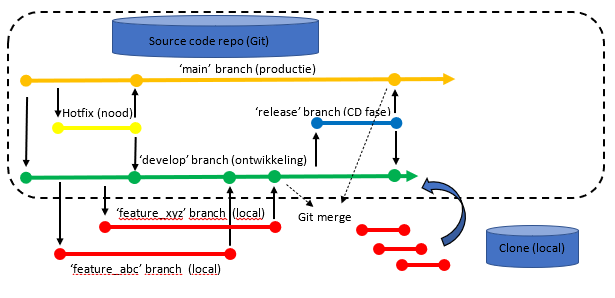
\includegraphics[scale=0.75]{Git_branching_strategy}
    \caption{Git branching strategie beschreven door Nelson Lopez}
    \label{fig:git branching strategie}
\end{figure}
\\ \\
De weg die een applicatie aflegt binnen de strategie die afgebeeld wordt op \ref{fig:git branching strategie} begint bij het binnenhalen van de applicatie versie die in de ontwikkelomgeving draait. Die is te vinden op de develop branch, vandaar wordt er een clone gemaakt naar een lokaal werkstation en wordt allereerst een nieuwe feature branch aangemaakt. De naamgeving van die branch kan als volgt zijn: feature-array-toevoegen, dit is afhankelijk van de policy binnen de werkomgeving omtrent naamgeving van branches.
\\ \\
Eenmaal de feature branch aangemaakt is kan de ontwikkelaar aan het werk gaan om de feature te coderen. In de tussentijd kan er een andere ontwikkelaar aan hetzelfde programma werken op nog een andere feature branch. Die ontwikkelaar moet bijvoorbeeld foutmeldingen aanpassen dus zijn feature branch krijgt de naam feature-update-foutmeldingen. Als een ontwikkelaar klaar is met zijn feature dan kan die een merge uitvoeren naar de develop branch om de versie die daar draait te updaten met zijn aangepaste versie. Doordat Git een merge functie heeft gaat Git enkel hetgeen aanpassen dat de ontwikkelaar zelf heeft gewijzigd. Zo kan er tussendoor iemand anders al een merge uitgevoerd hebben naar diezelfde branch zonder dat er conflicten zijn.
\\ \\
Nadat een applicatie in de ontwikkelomgeving een of meerdere updates heeft gekregen kan er gekozen worden om die versie over te zetten naar de productie omgeving. Voordat effectief plaatsvindt zal er eerst een release branch aangemaakt worden om de functionele testen uit te voeren en indien nodig source code aan te passen. Pas als de testen vlot verlopen dan wordt er zowel met de main branch (productie) als met de develop branch een merge uitgevoerd. Zo zijn beide versies up to date met de versie die doorheen de functionele test fase is geraakt (QA).
\\ \\
In geval dat er een situatie is waarin de productie versie niet meer draait dan wordt er een hotfix branch gemaakt vanaf de versie die draait op productie. Source code wordt aangepast en testing wordt opnieuw uitgevoerd zoals bij de release branch. Indien die testen succesvol zijn dan wordt de aangepaste versie zowel met de main branch als met de develop branch gemerged. Hierdoor wordt de fout die in de productie versie zat zowel in de ontwikkelomgeving als in de productieomgeving opgelost.
\\ \\